\chapter{Resultados de incertidumbre optimización Uniforme} \label{anx:uniforme}

\begin{figure}[ht]
    \centering
    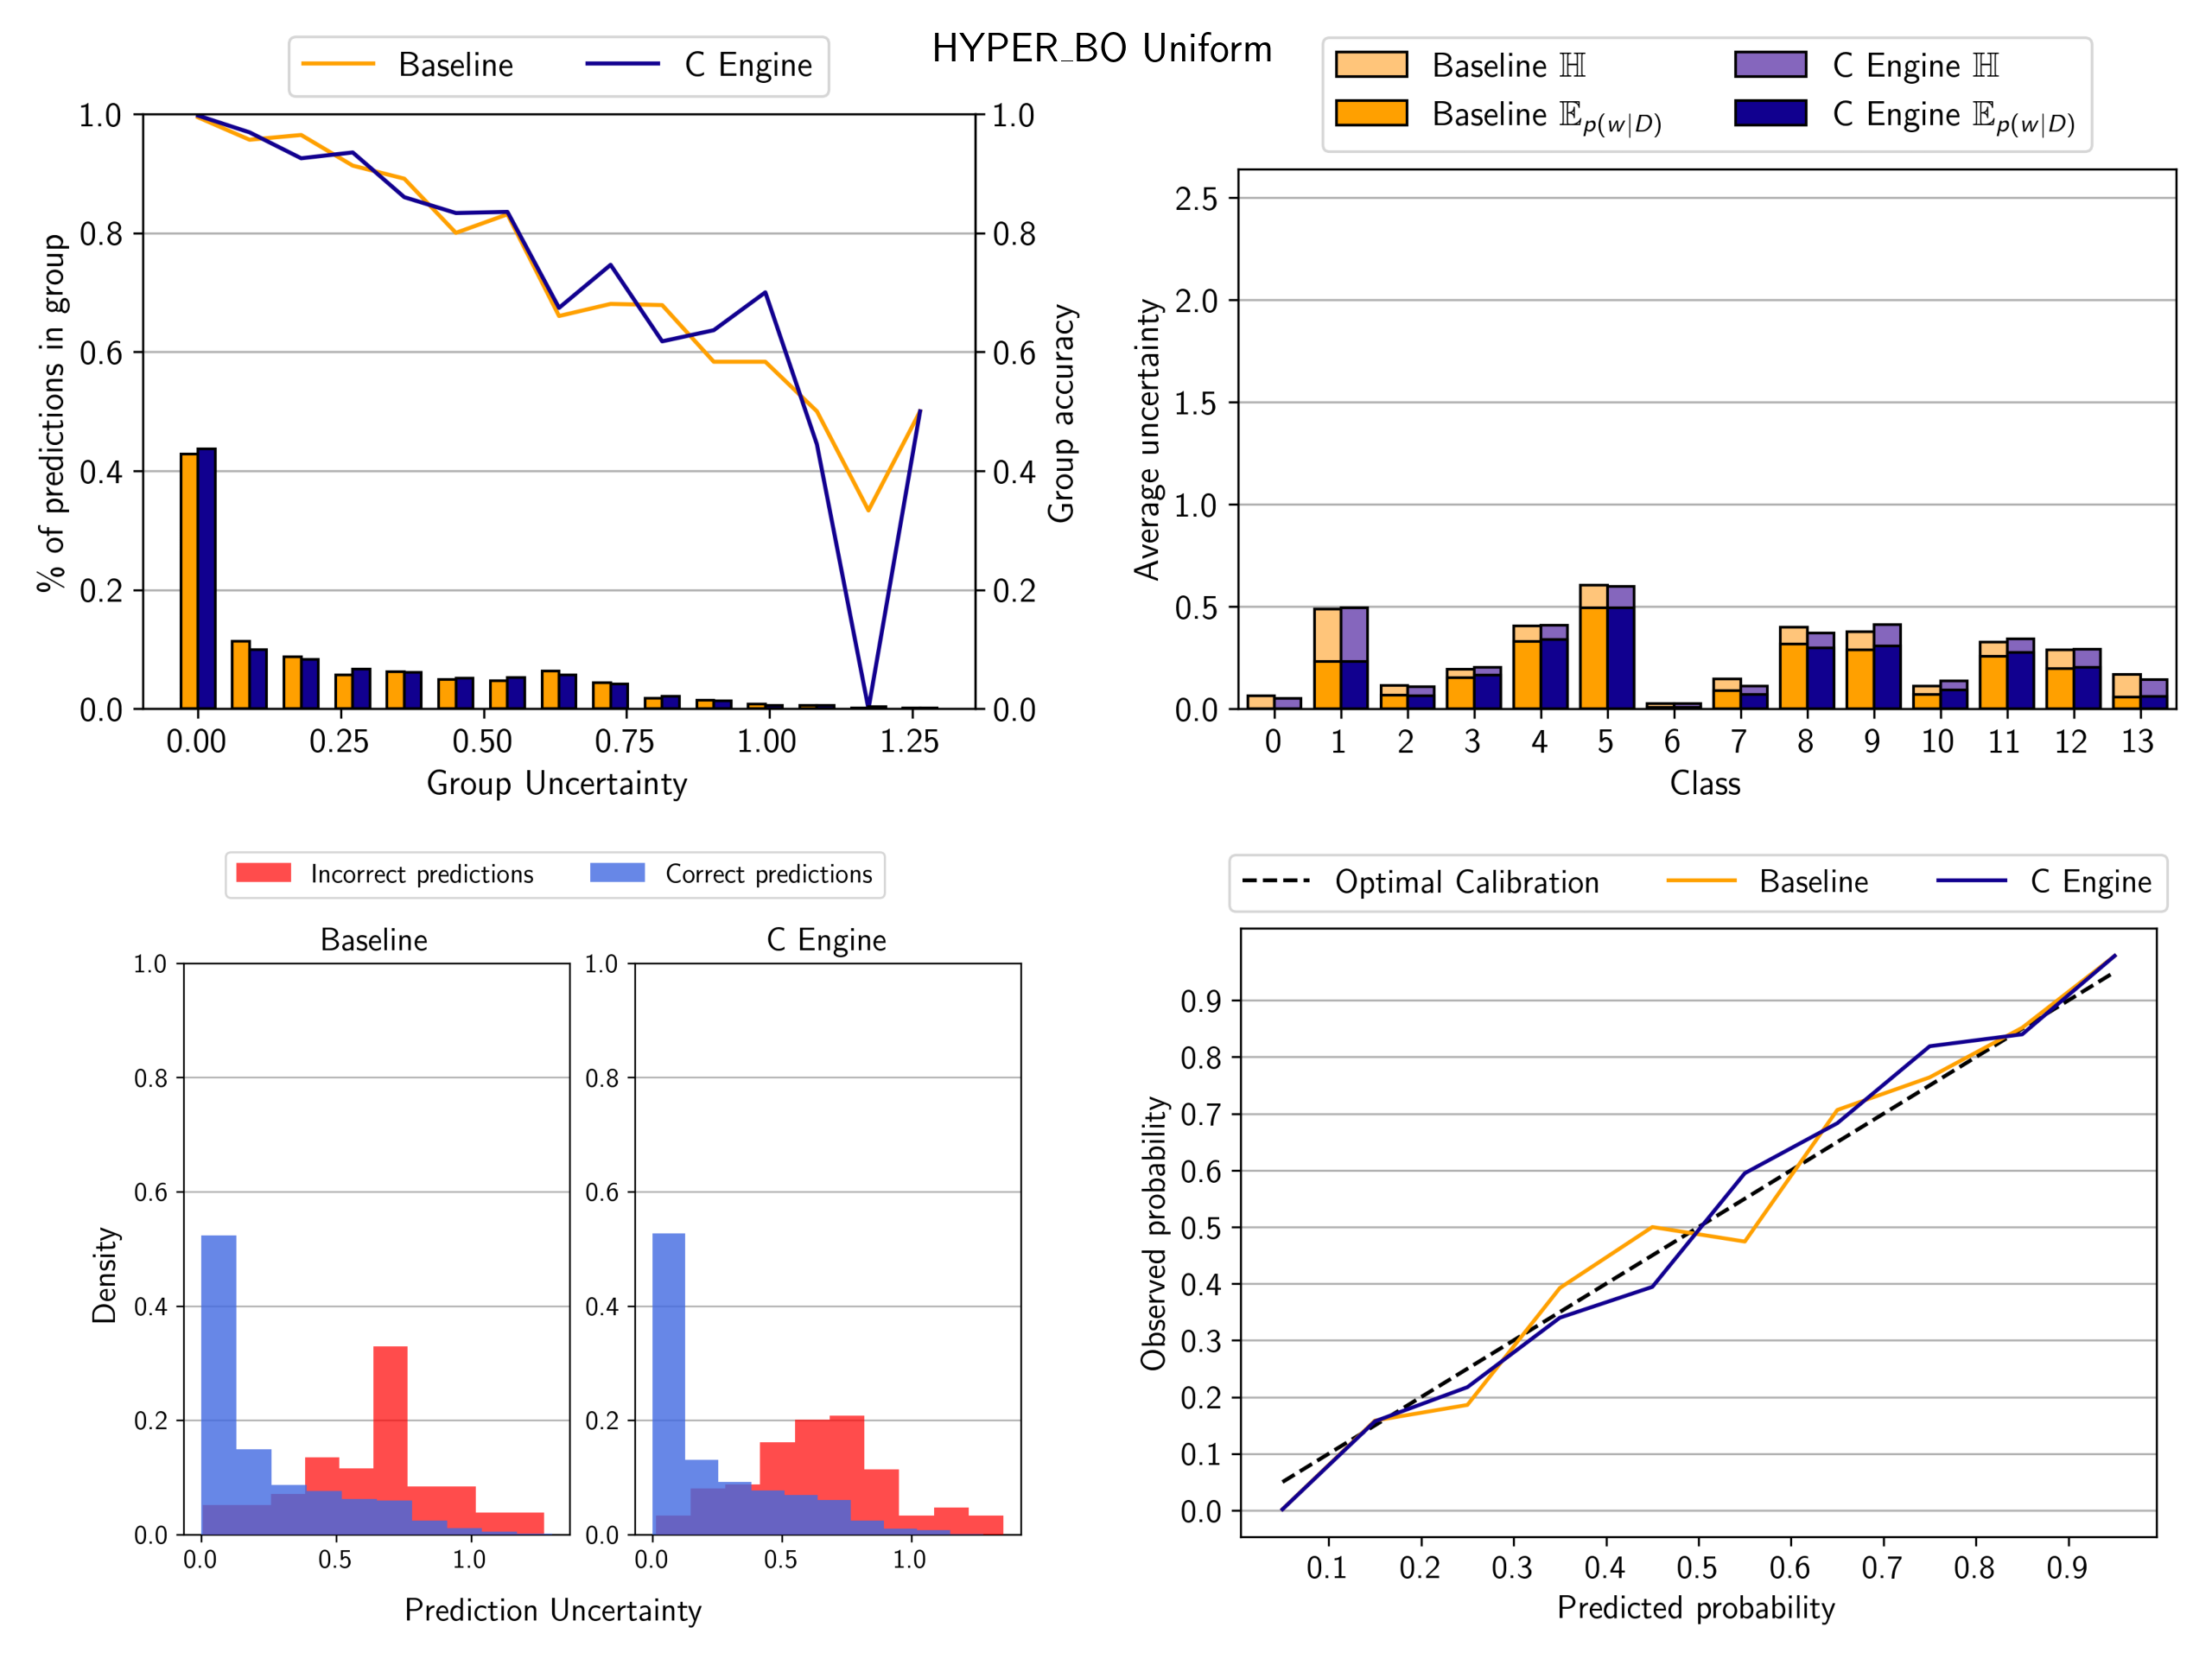
\includegraphics[width=0.9\textwidth]{root/Imagenes/anexo/Uniform-HYPER_BO-mosaic.png}
    \caption{Predicciones del conjunto de prueba de píxeles hiperespectrales BO.}
    \label{fig:anx-Uniform-HYPER_BO}
\end{figure}


\begin{figure}[ht]
    \centering
    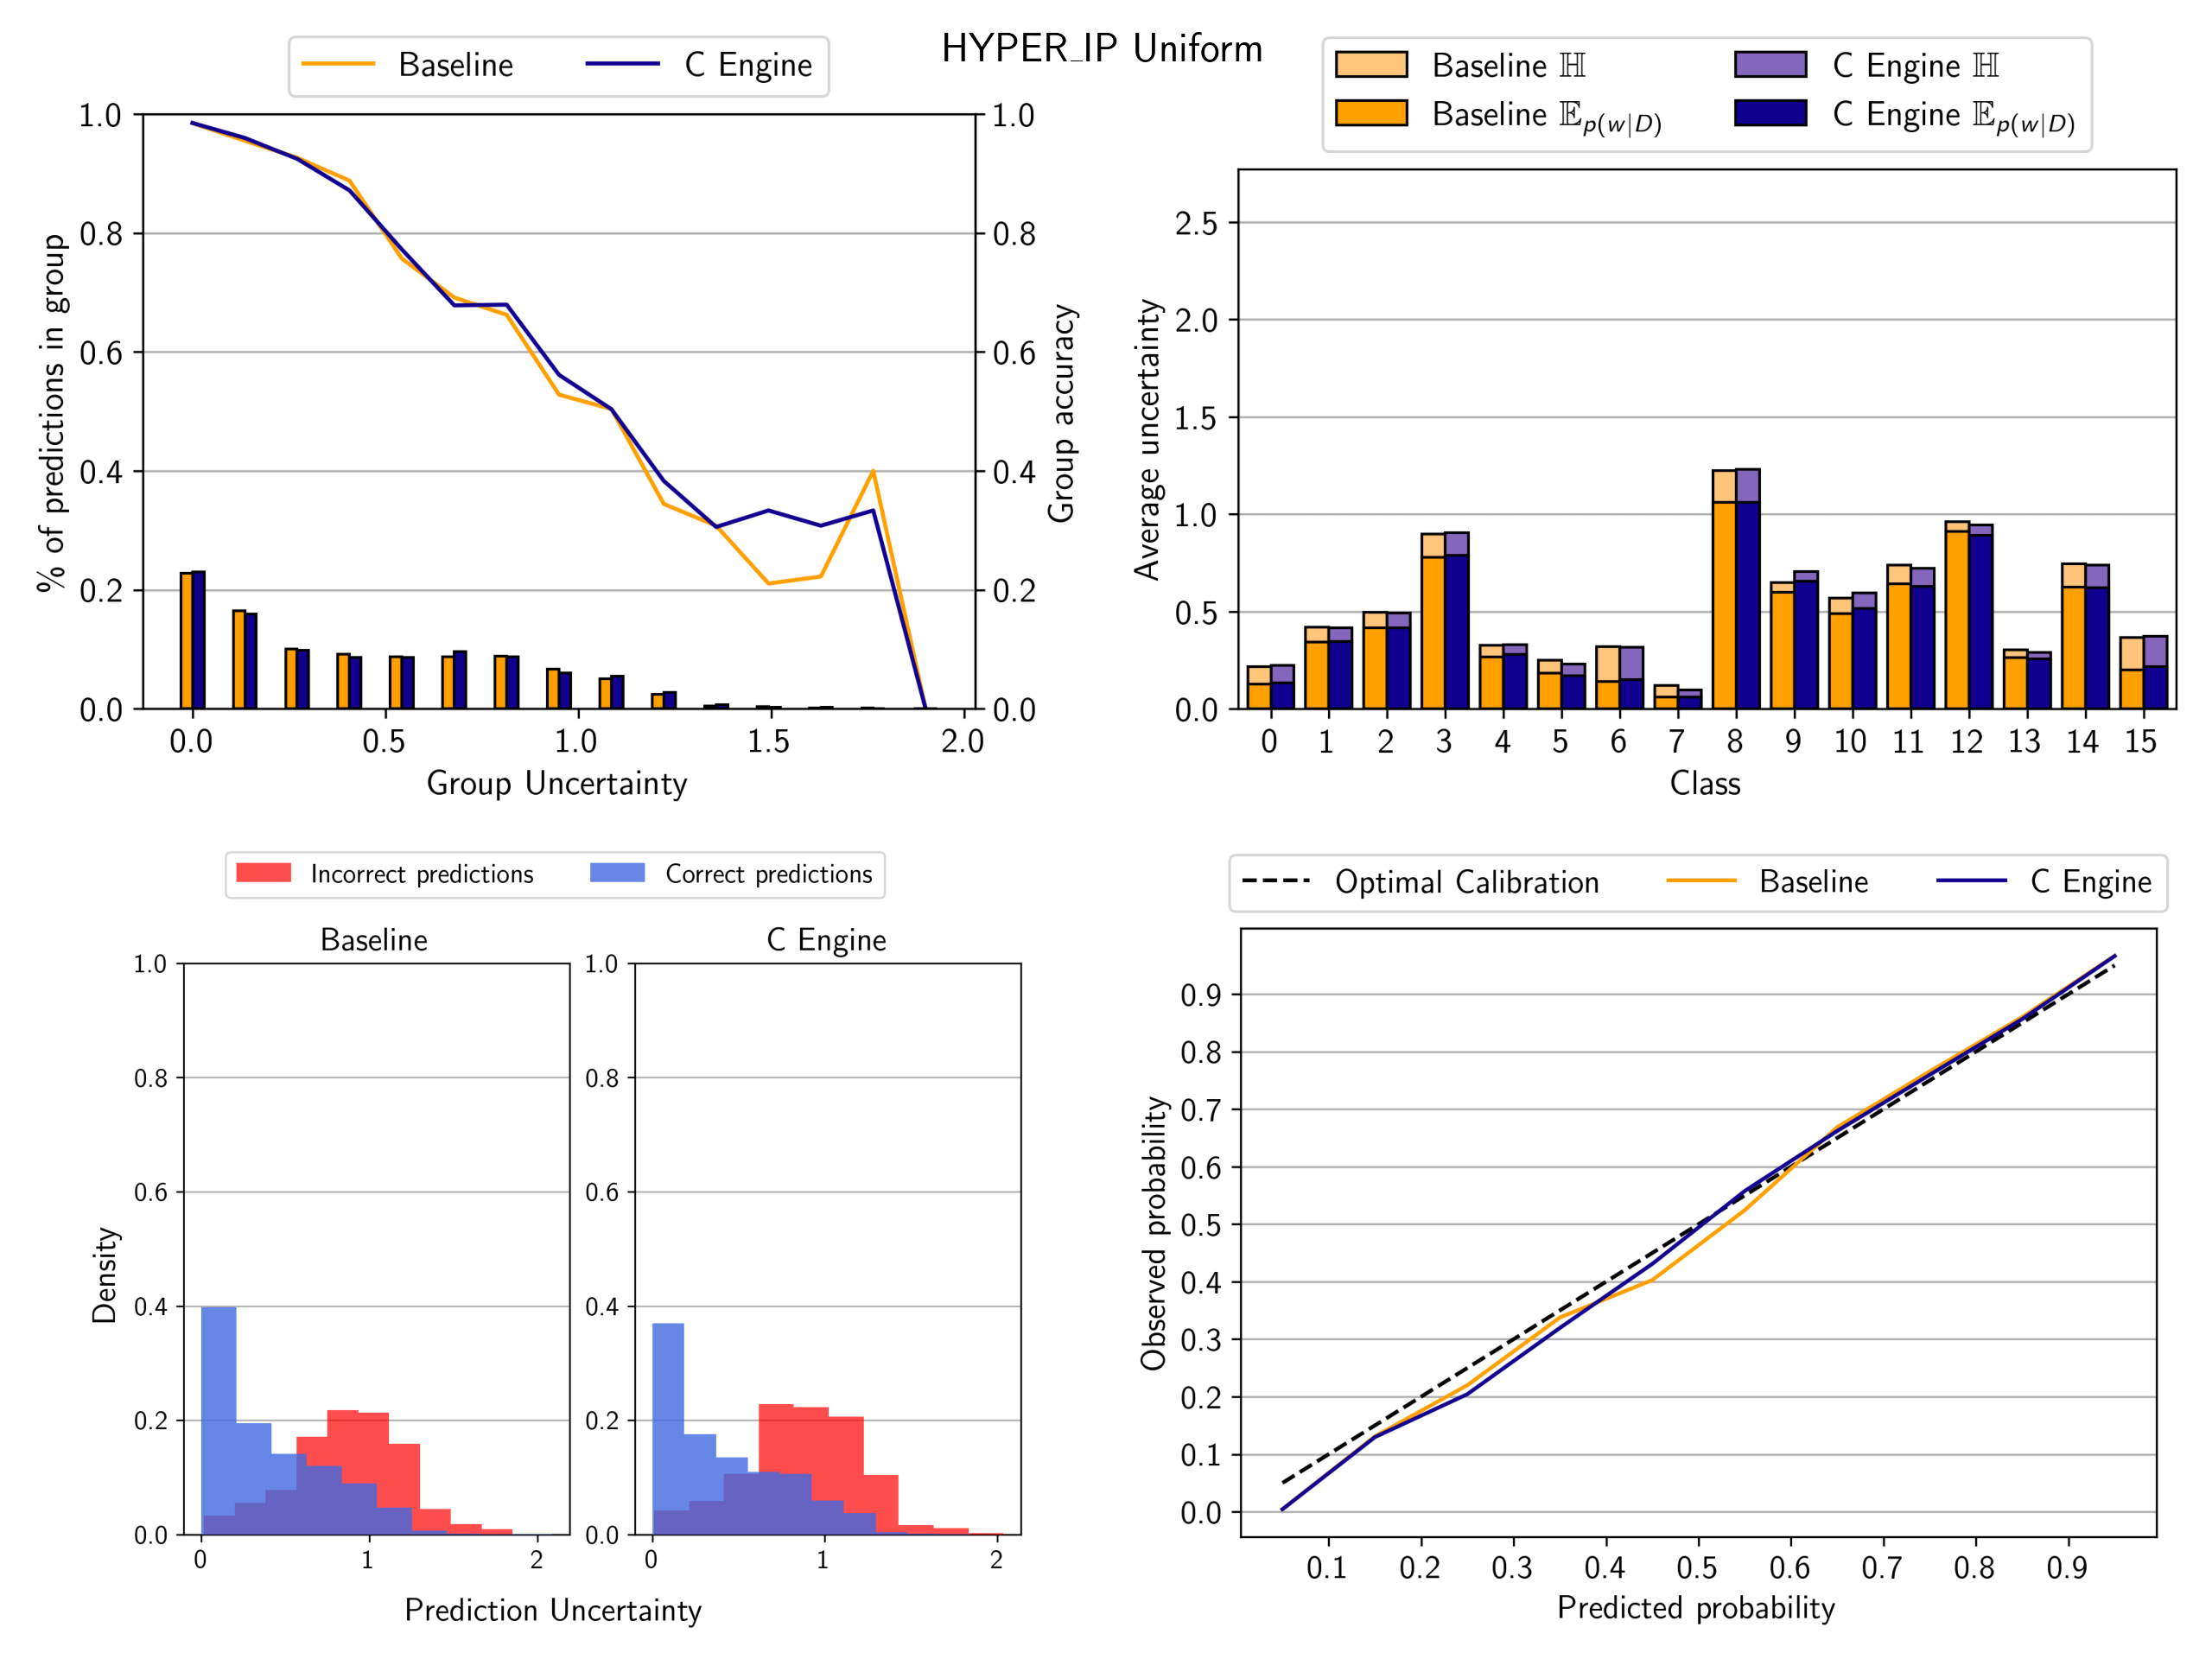
\includegraphics[width=0.9\textwidth]{root/Imagenes/anexo/Uniform-HYPER_IP-mosaic.png}
    \caption{Predicciones del conjunto de prueba de píxeles hiperespectrales IP.}
    \label{fig:anx-Uniform-HYPER_IP}
\end{figure}


\begin{figure}[ht]
    \centering
    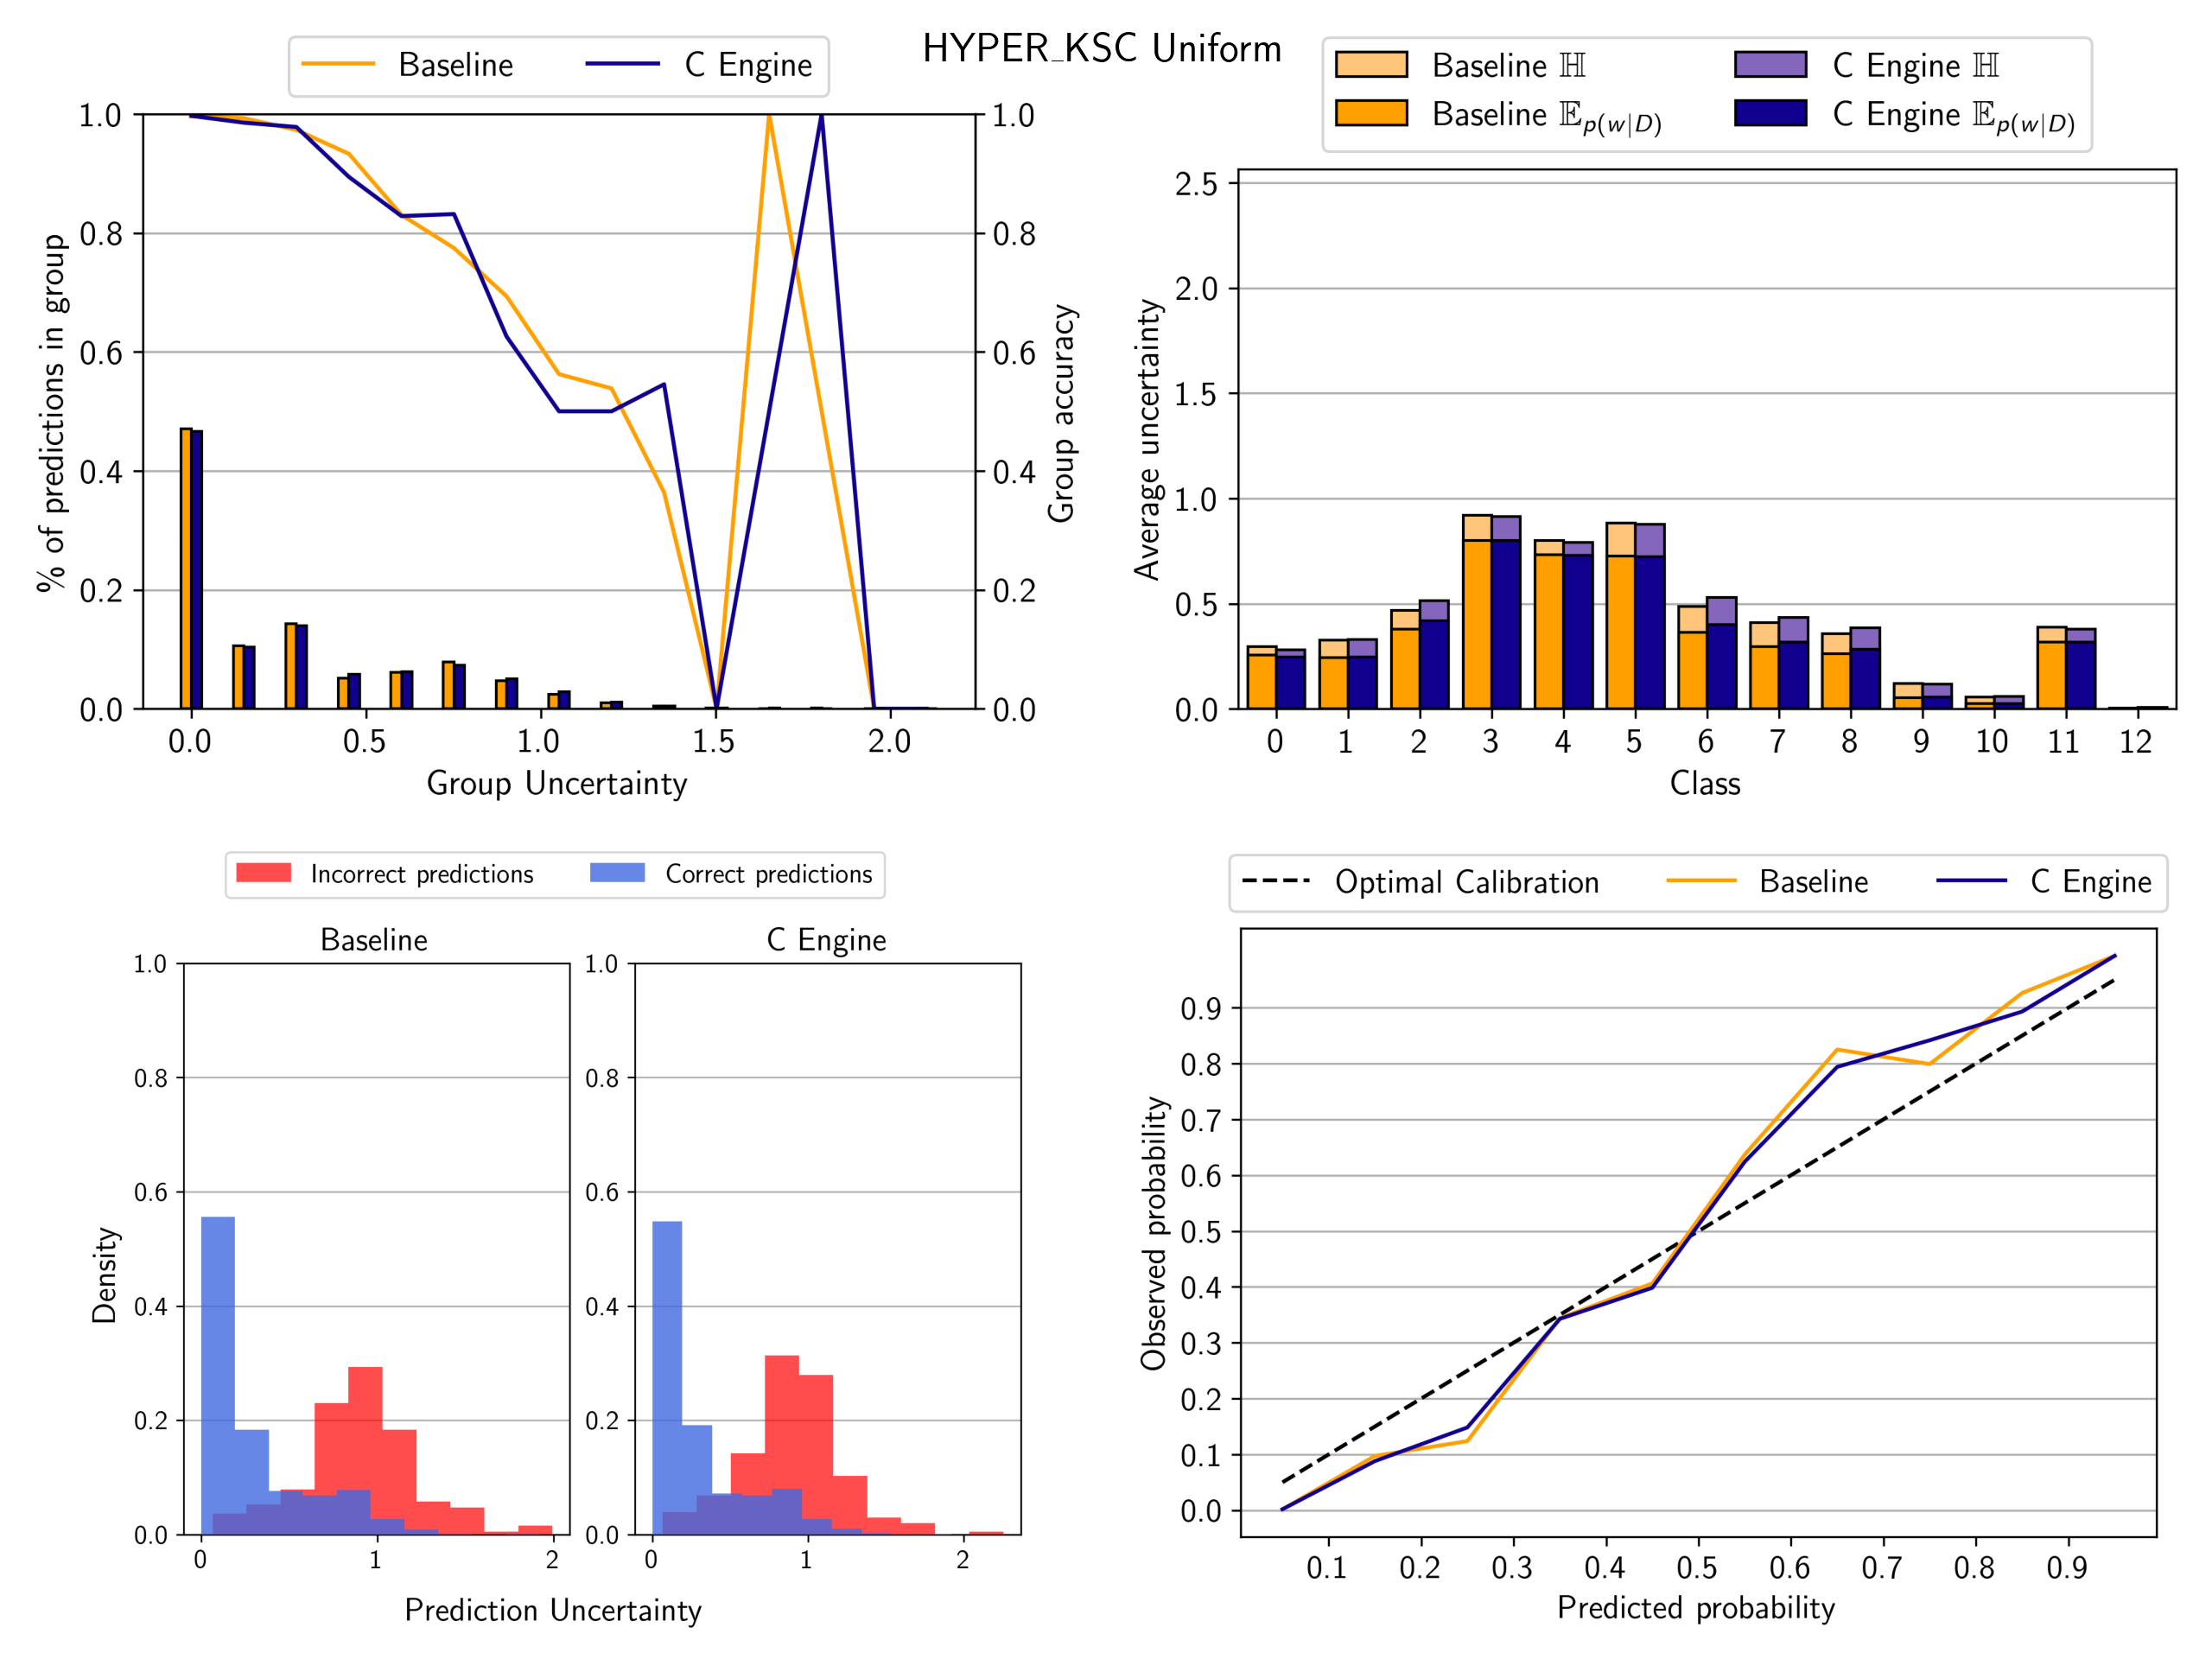
\includegraphics[width=0.9\textwidth]{root/Imagenes/anexo/Uniform-HYPER_KSC-mosaic.png}
    \caption{Predicciones del conjunto de prueba de píxeles hiperespectrales KSC.}
    \label{fig:anx-Uniform-HYPER_KSC}
\end{figure}


\begin{figure}[ht]
    \centering
    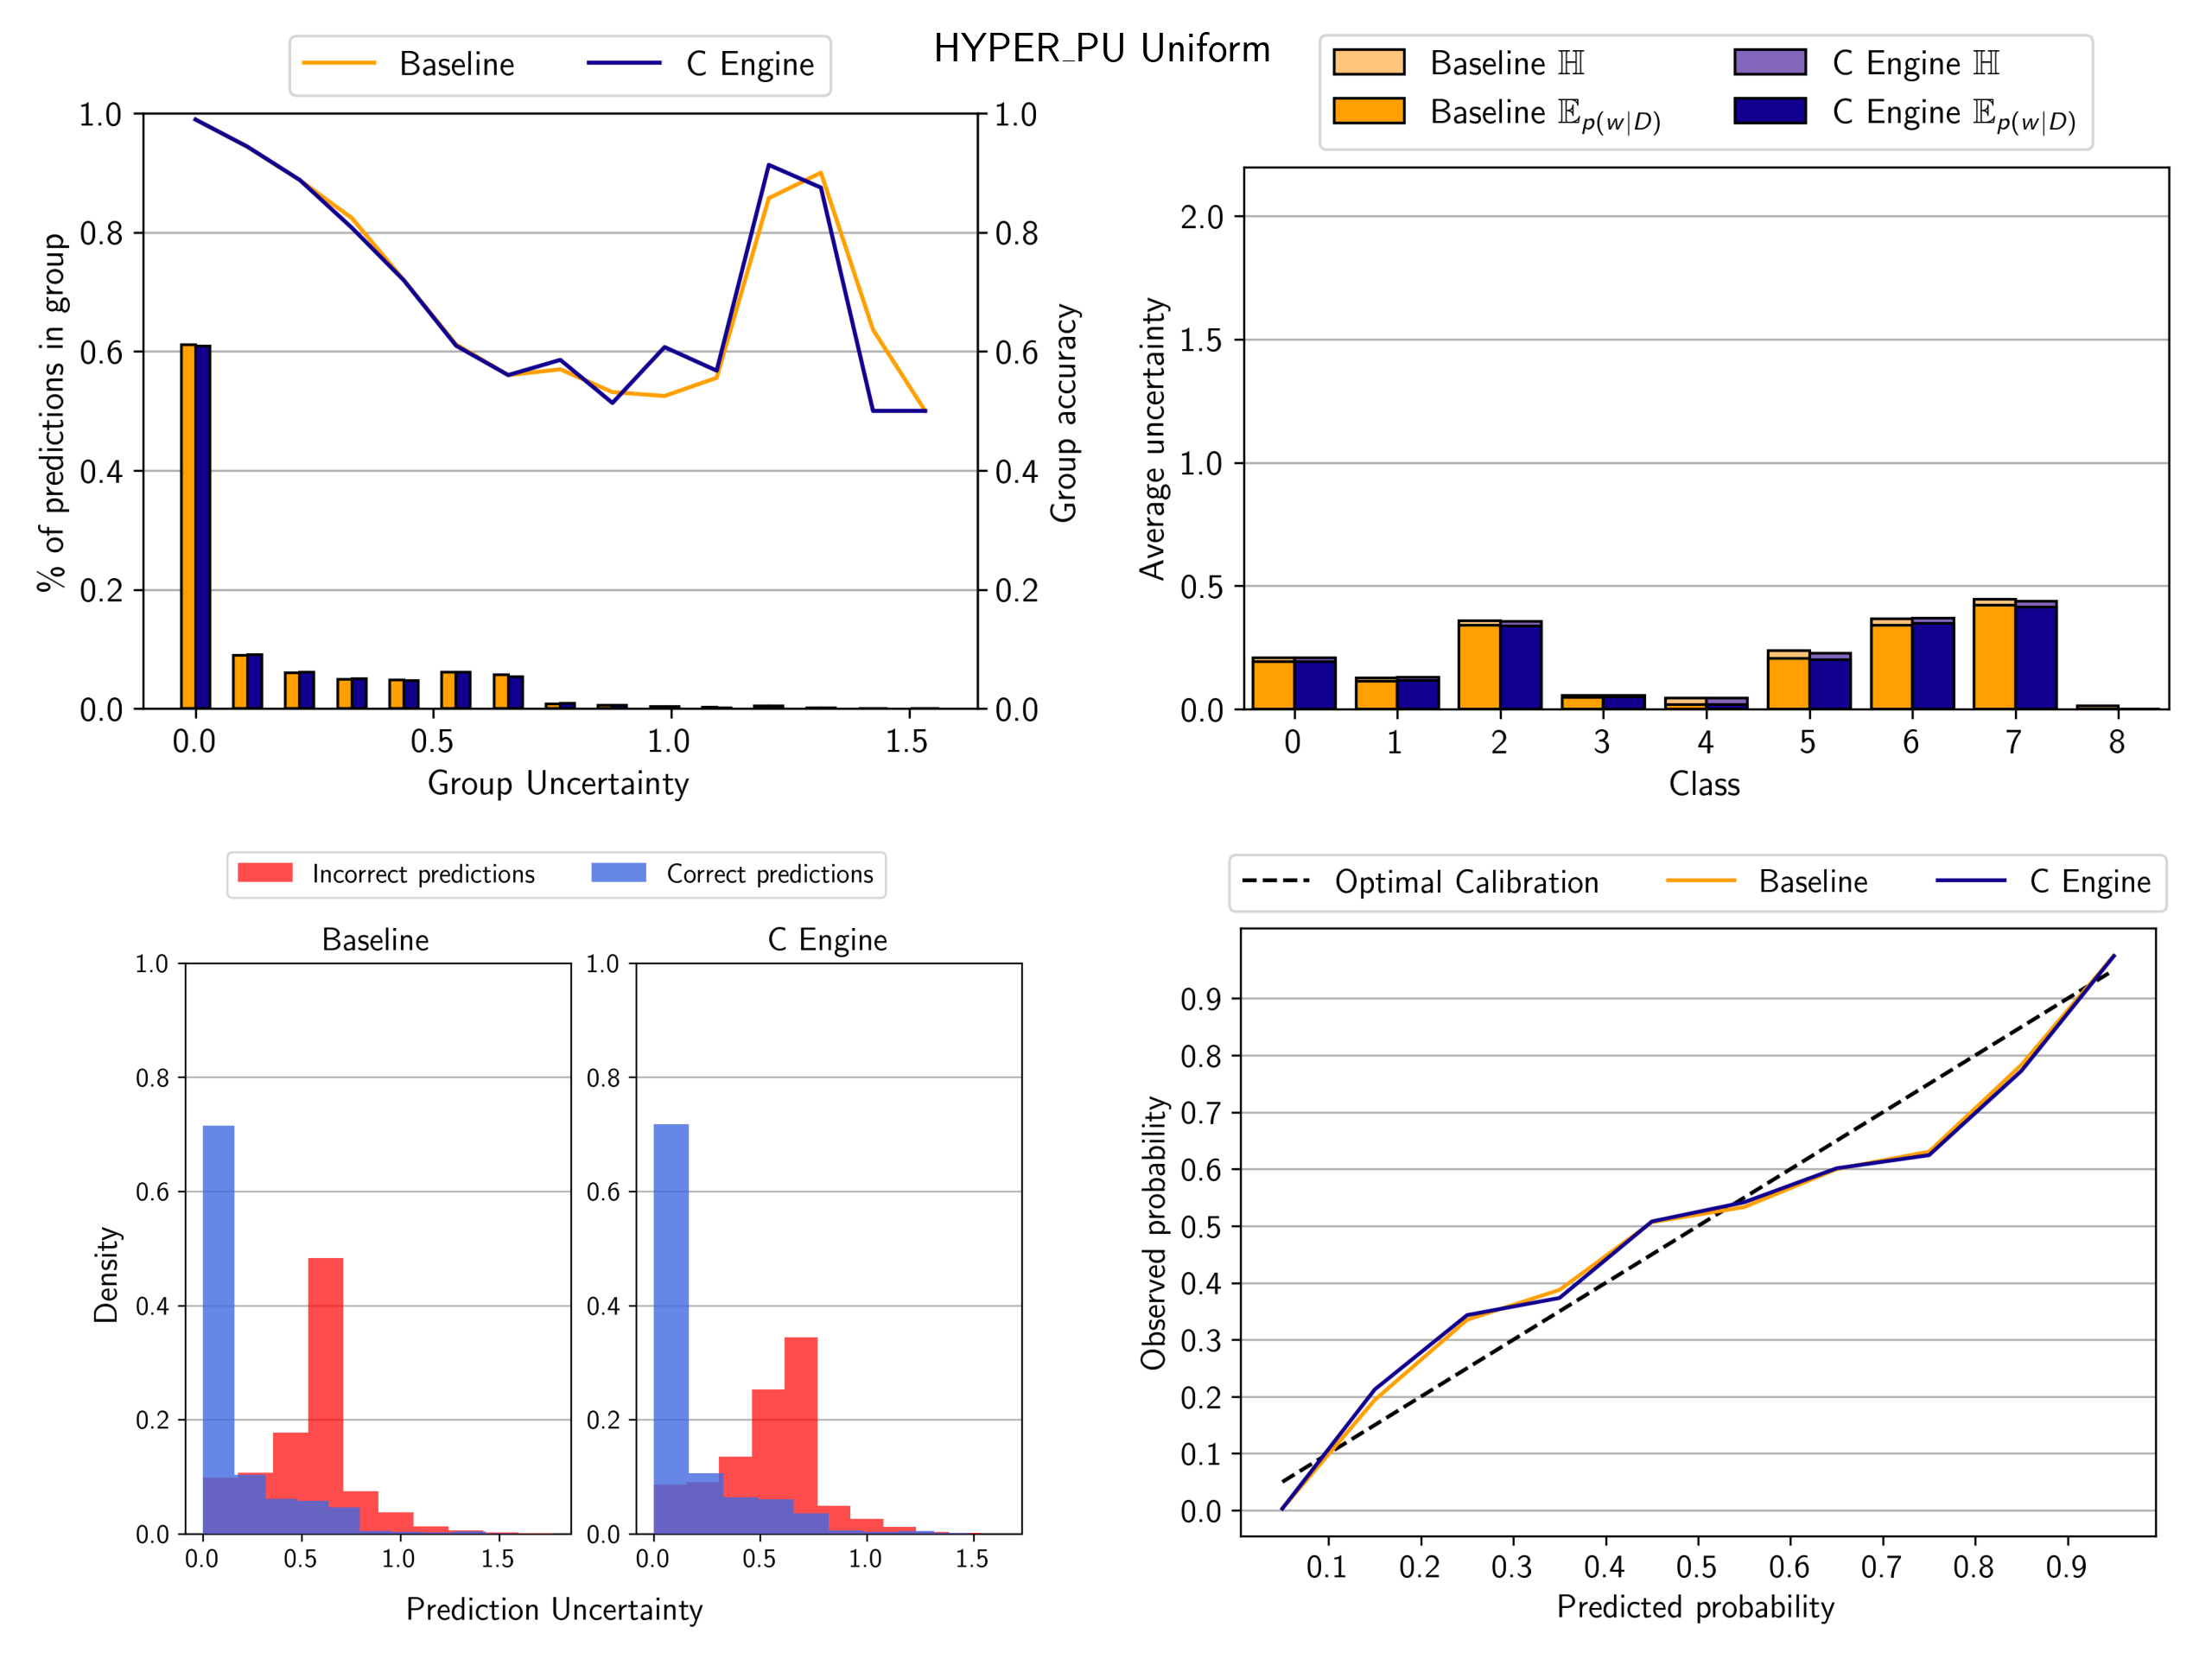
\includegraphics[width=0.9\textwidth]{root/Imagenes/anexo/Uniform-HYPER_PU-mosaic.png}
    \caption{Predicciones del conjunto de prueba de píxeles hiperespectrales PU.}
    \label{fig:anx-Uniform-HYPER_PU}
\end{figure}


\begin{figure}[ht]
    \centering
    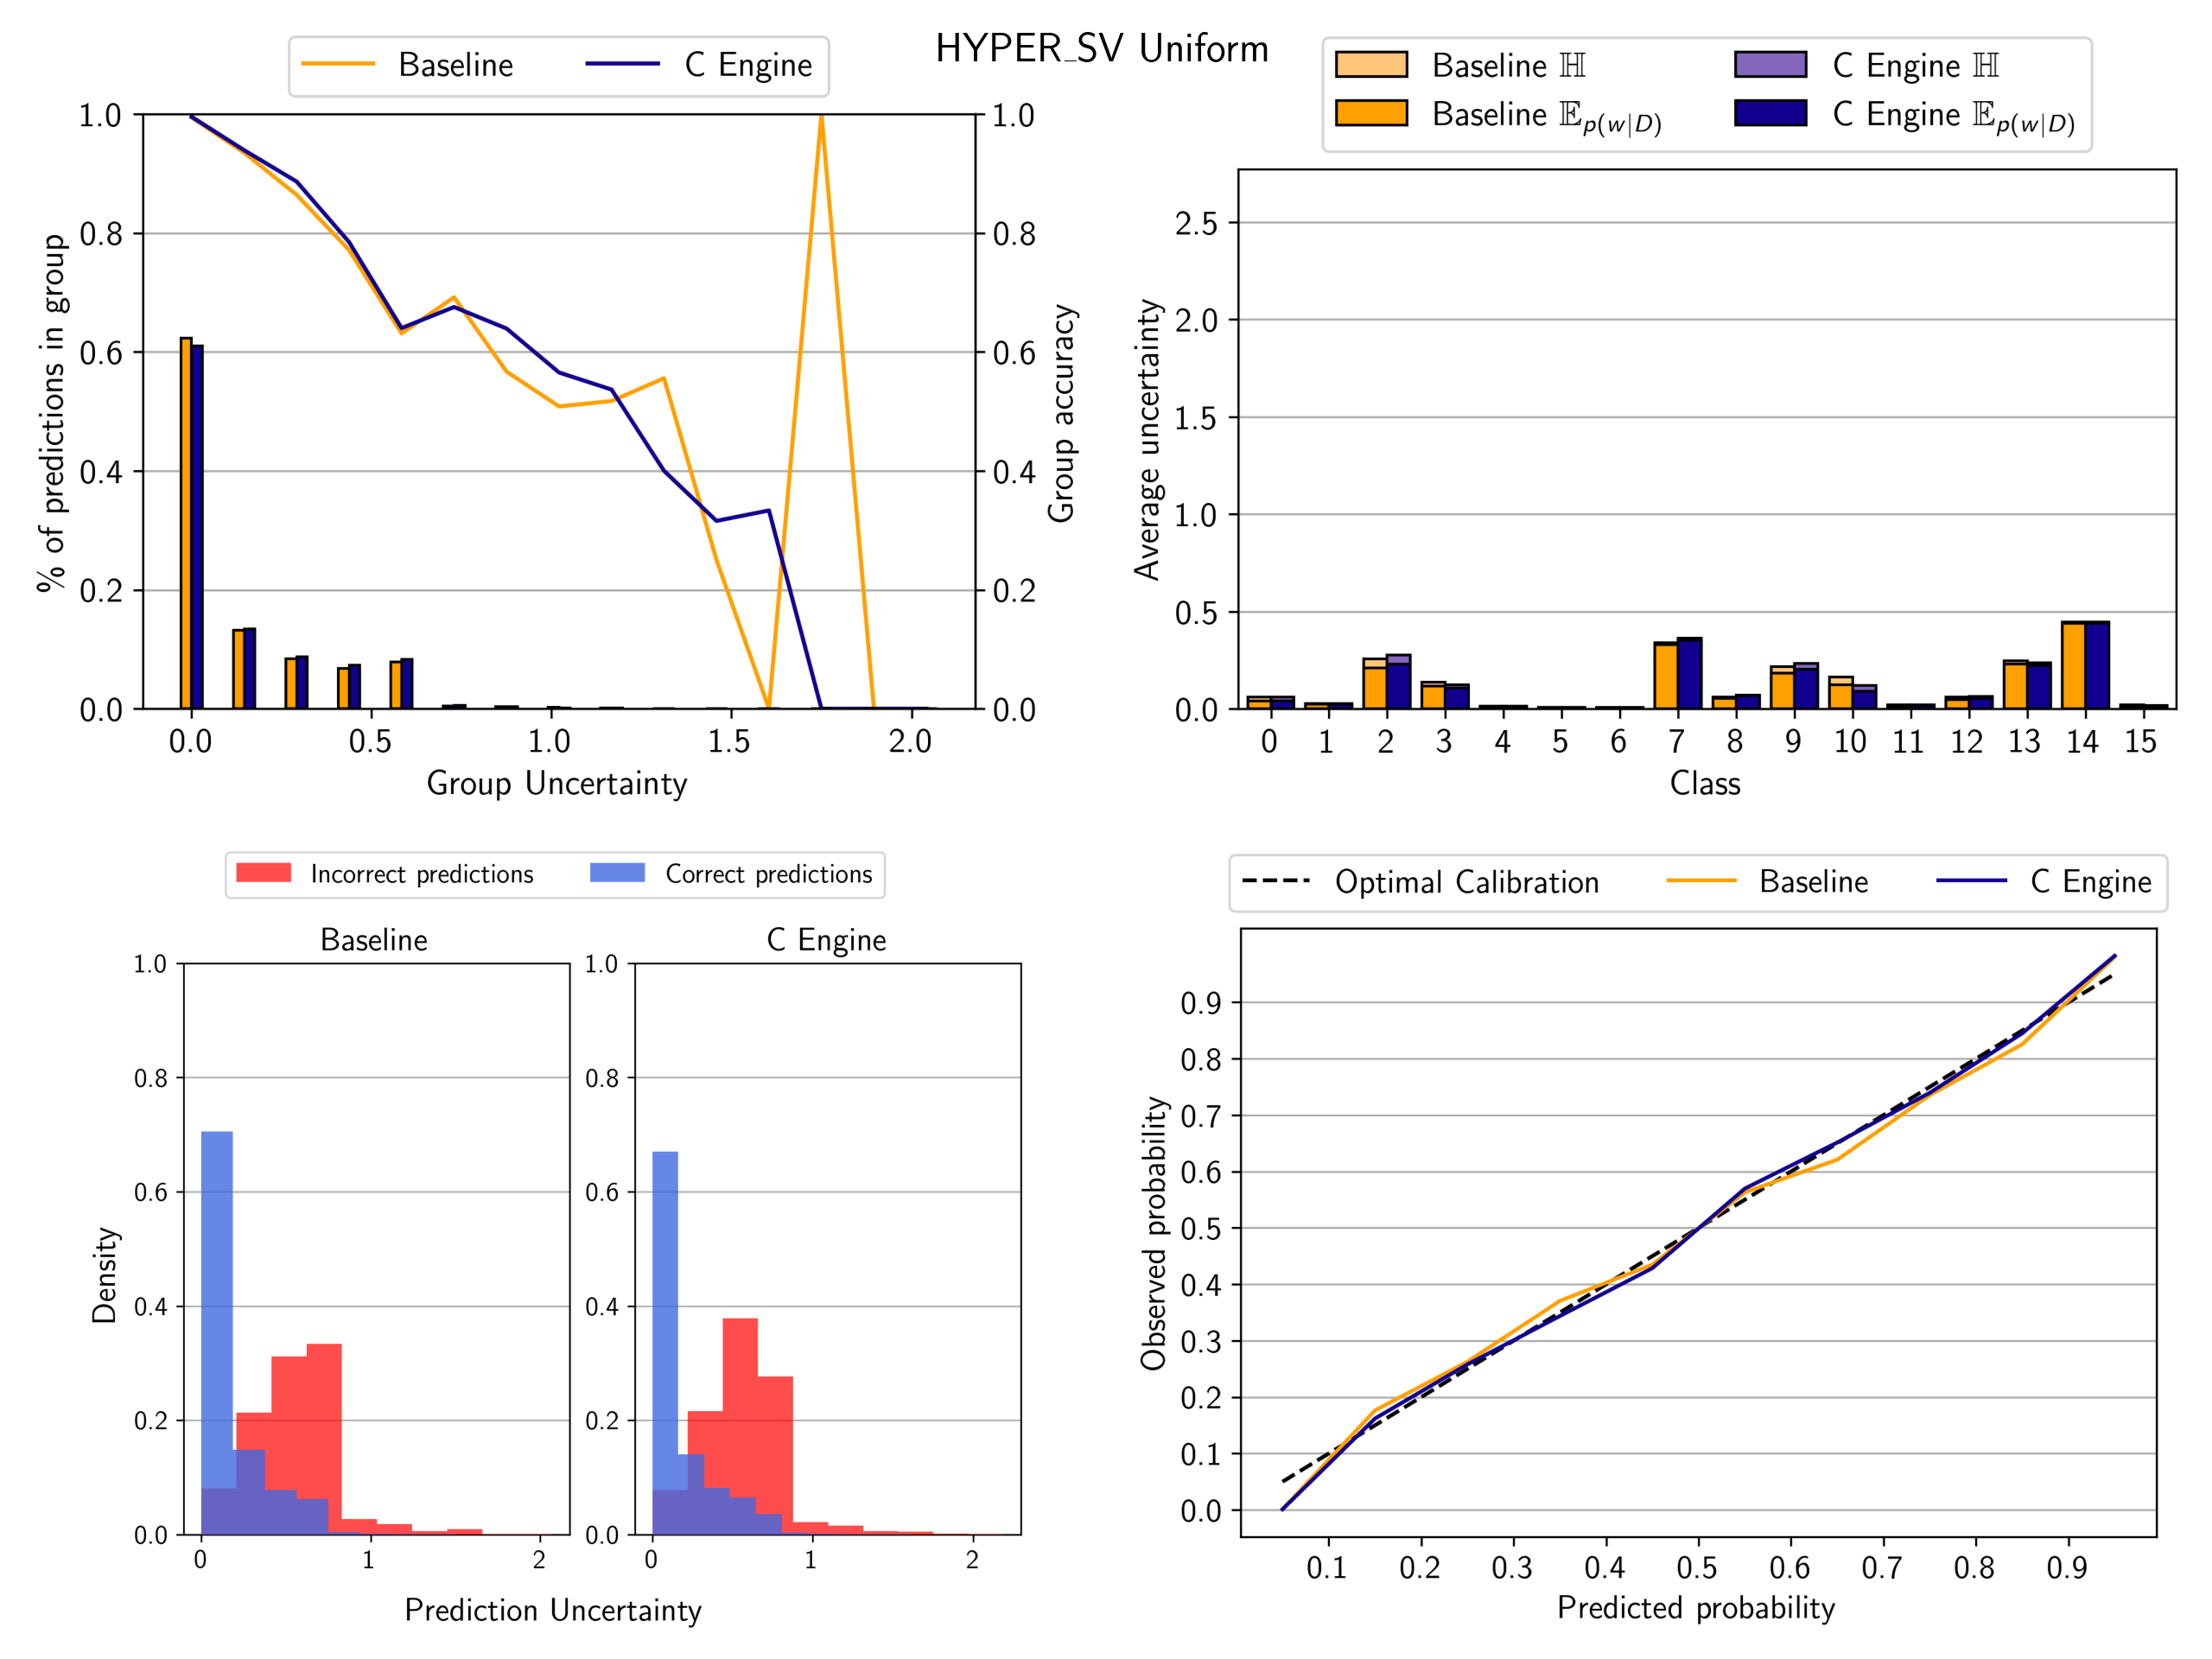
\includegraphics[width=0.9\textwidth]{root/Imagenes/anexo/Uniform-HYPER_SV-mosaic.png}
    \caption{Predicciones del conjunto de prueba de píxeles hiperespectrales SV.}
    \label{fig:anx-Uniform-HYPER_SV}
\end{figure}


\begin{figure}[ht]
    \centering
    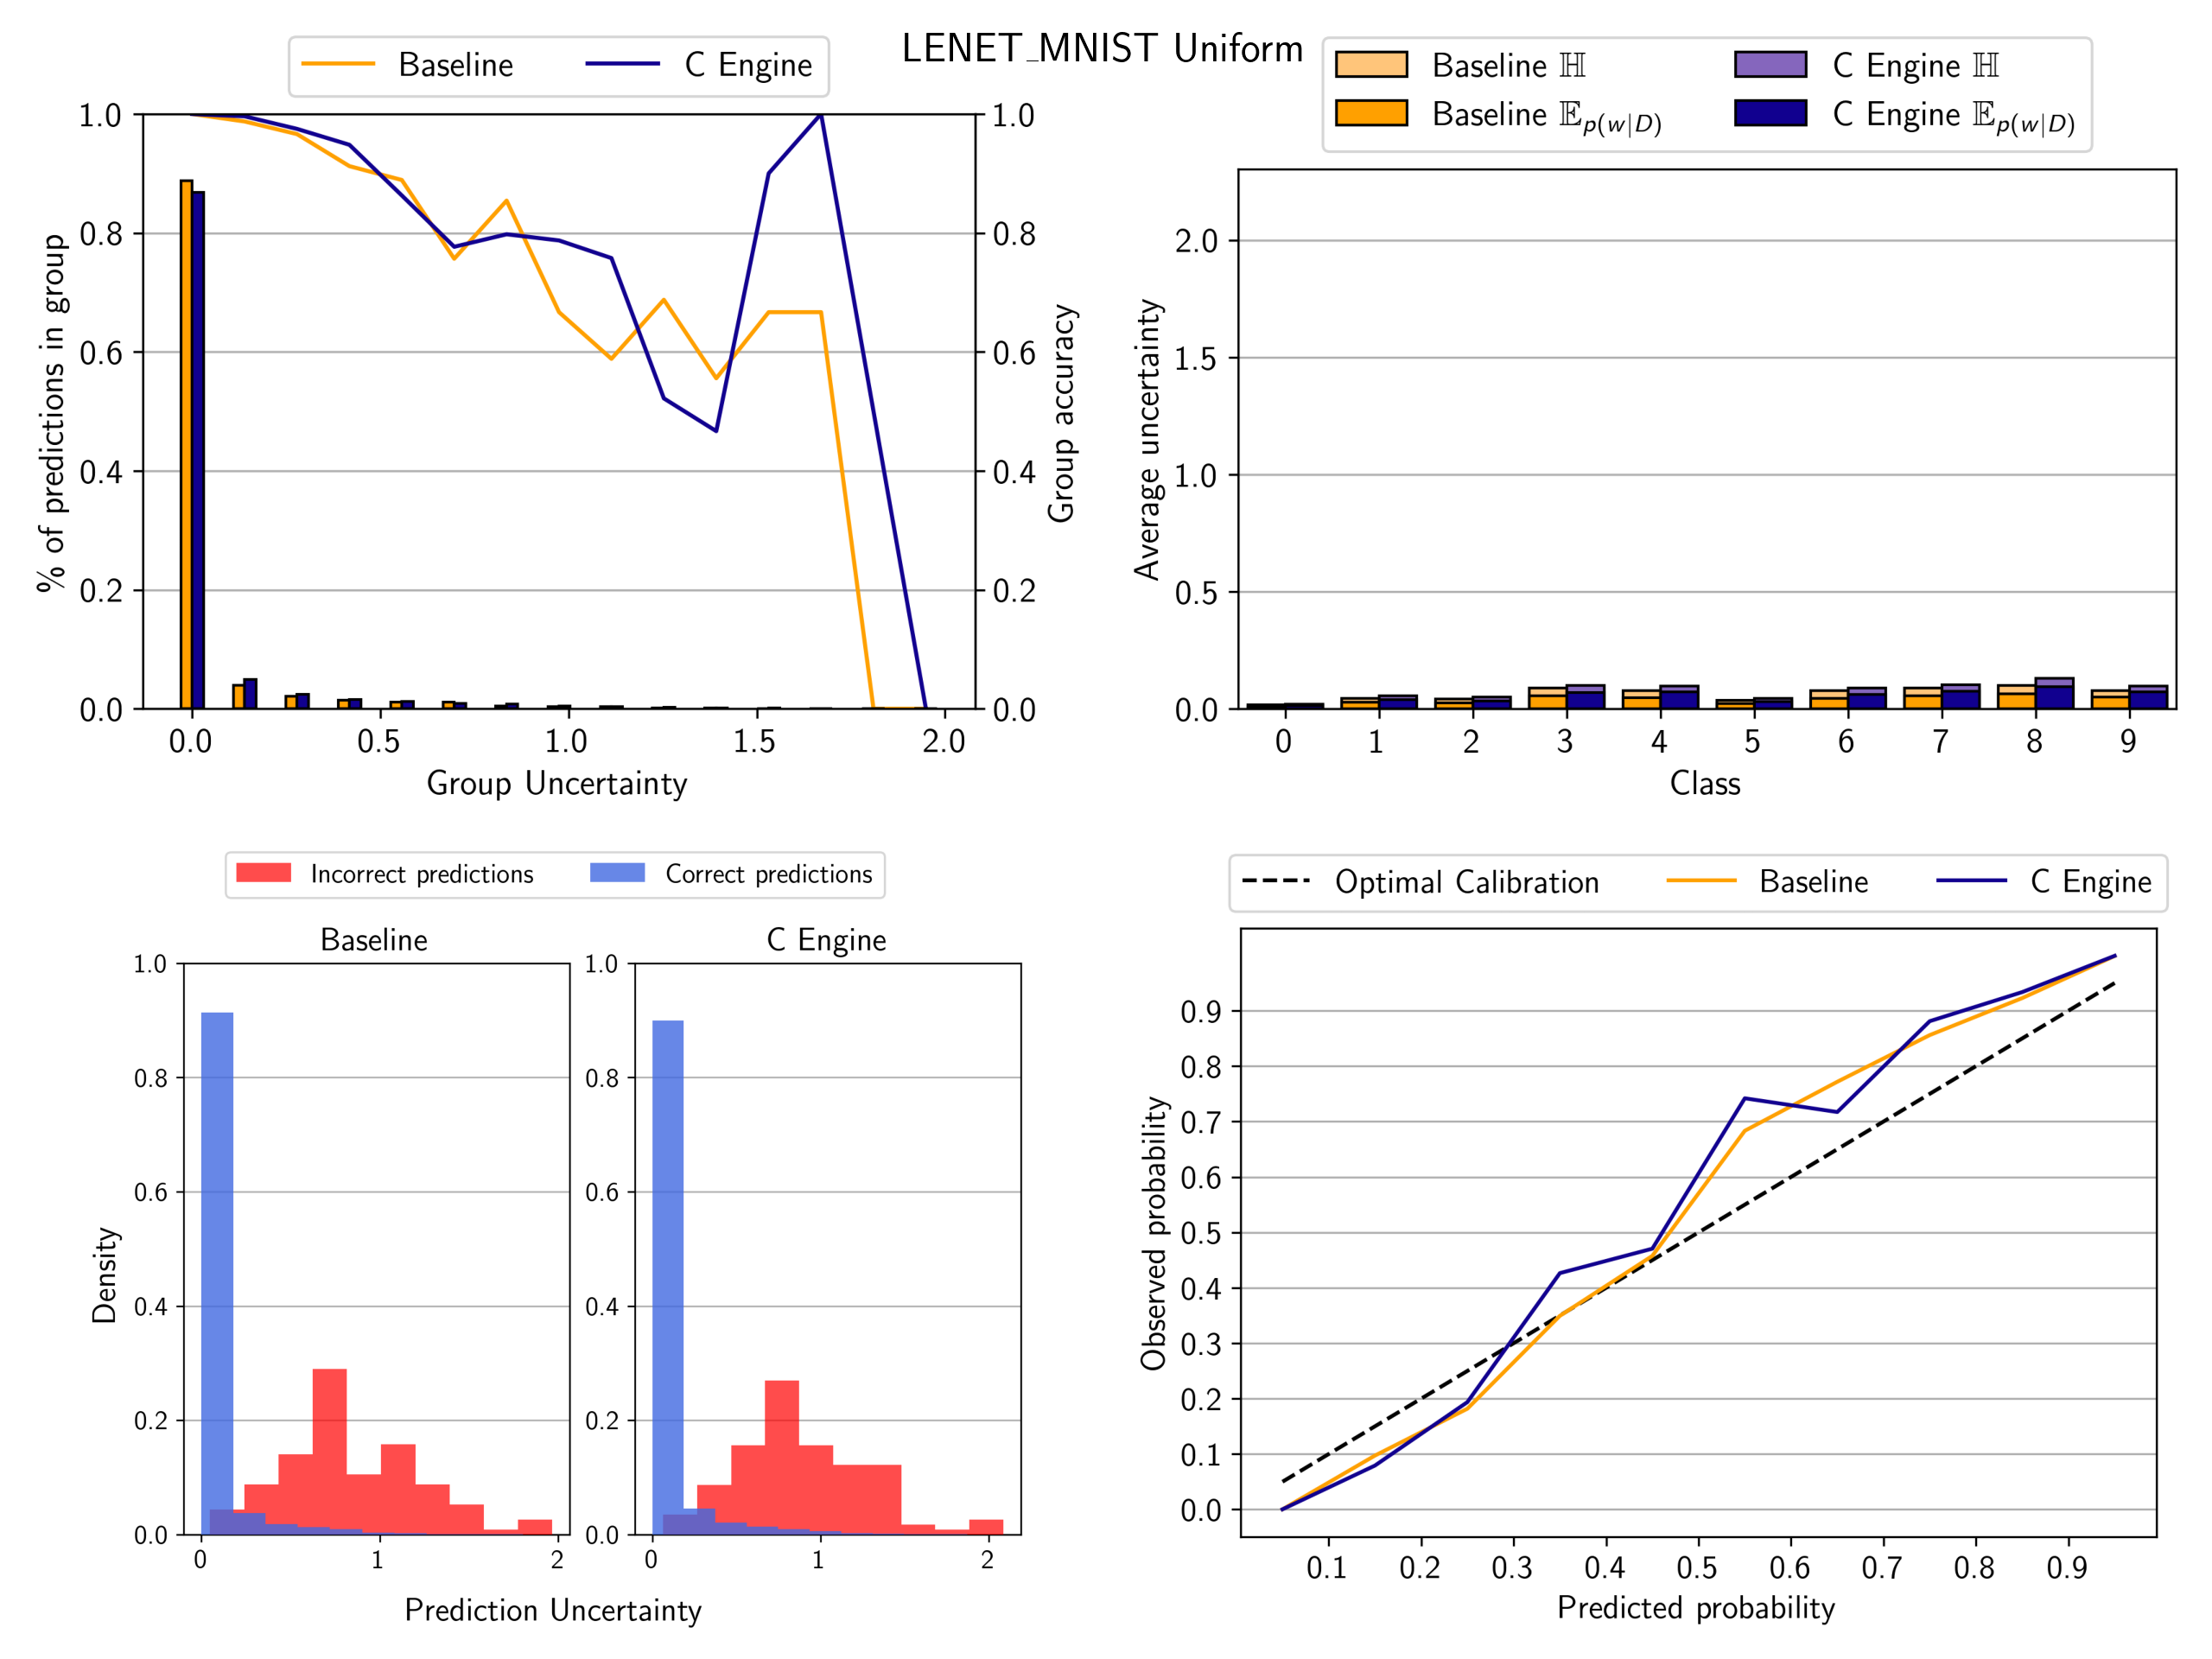
\includegraphics[width=0.9\textwidth]{root/Imagenes/anexo/Uniform-LENET_MNIST-mosaic.png}
    \caption{Predicciones del modelo LENET con el conjunto de datos MNIST.}
    \label{fig:anx-Uniform-LENET_MNIST}
\end{figure}


\begin{figure}[ht]
    \centering
    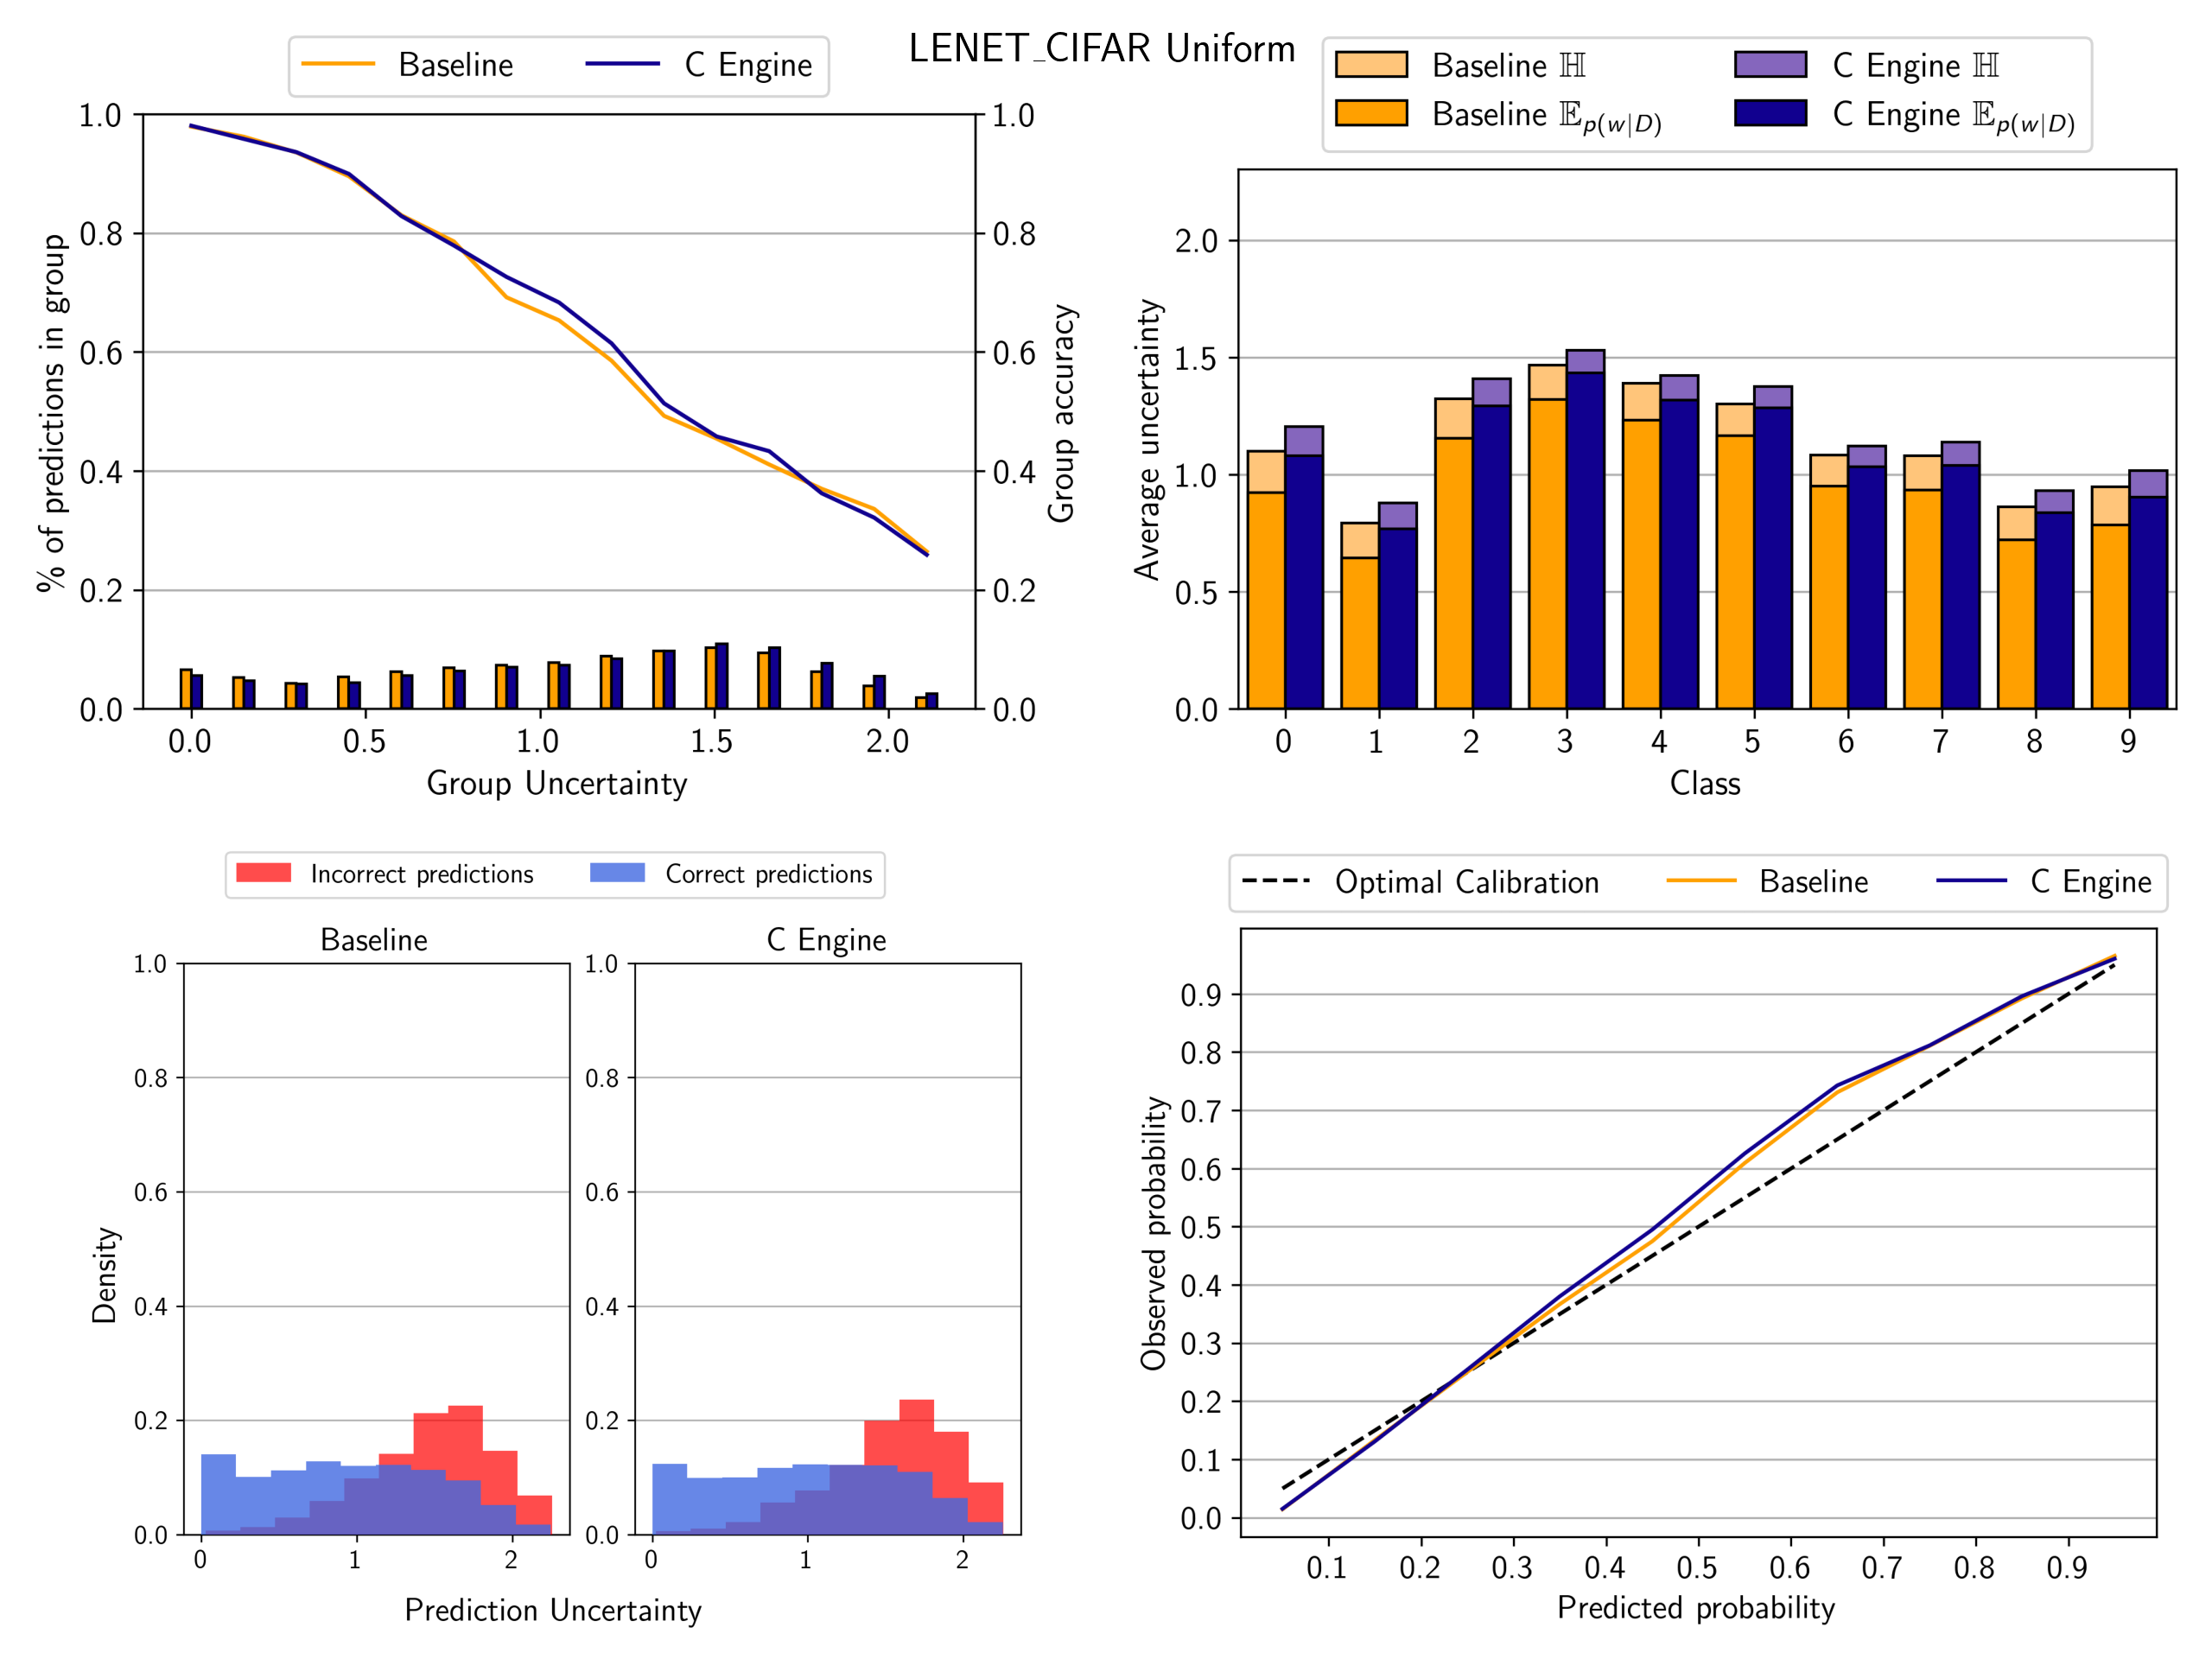
\includegraphics[width=0.9\textwidth]{root/Imagenes/anexo/Uniform-LENET_CIFAR-mosaic.png}
    \caption{Predicciones del modelo LENET con el conjunto de datos CIFAR-10.}
    \label{fig:anx-Uniform-LENET_CIFAR}
\end{figure}


\begin{figure}[ht]
    \centering
    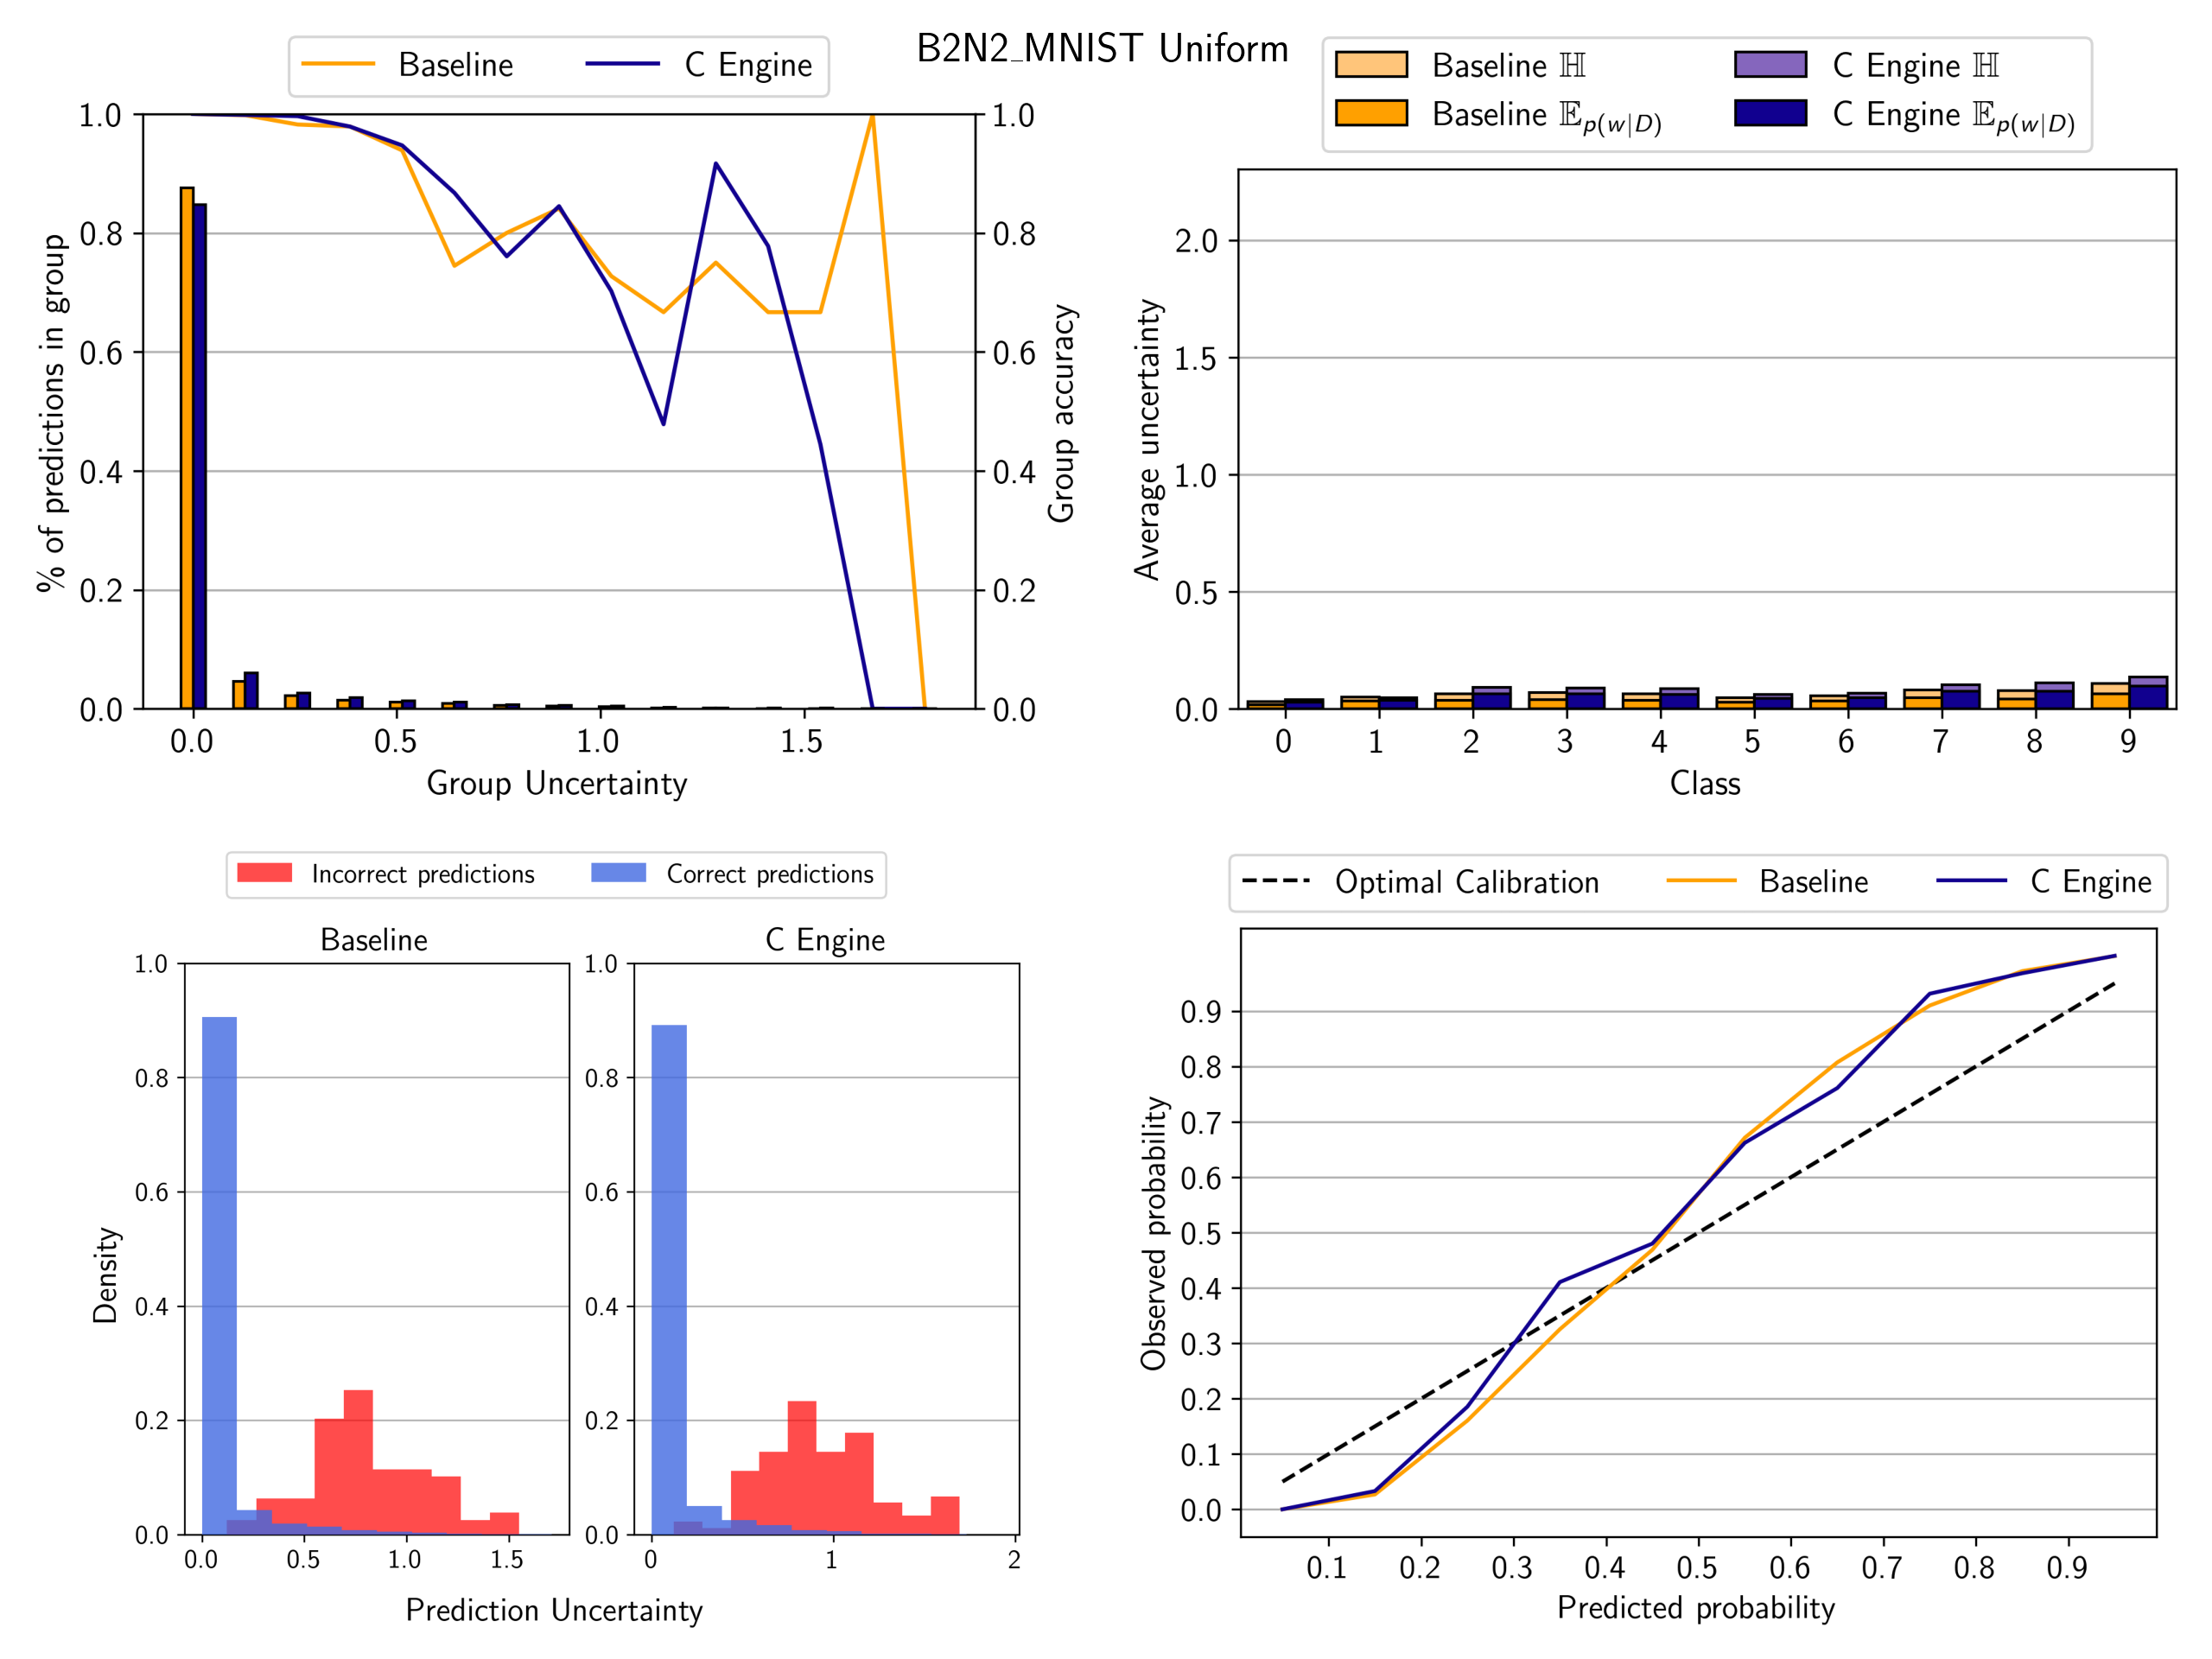
\includegraphics[width=0.9\textwidth]{root/Imagenes/anexo/Uniform-B2N2_MNIST-mosaic.png}
    \caption{Predicciones del modelo B2N2 con el conjunto de datos MNIST.}
    \label{fig:anx-Uniform-B2N2_MNIST}
\end{figure}


\begin{figure}[ht]
    \centering
    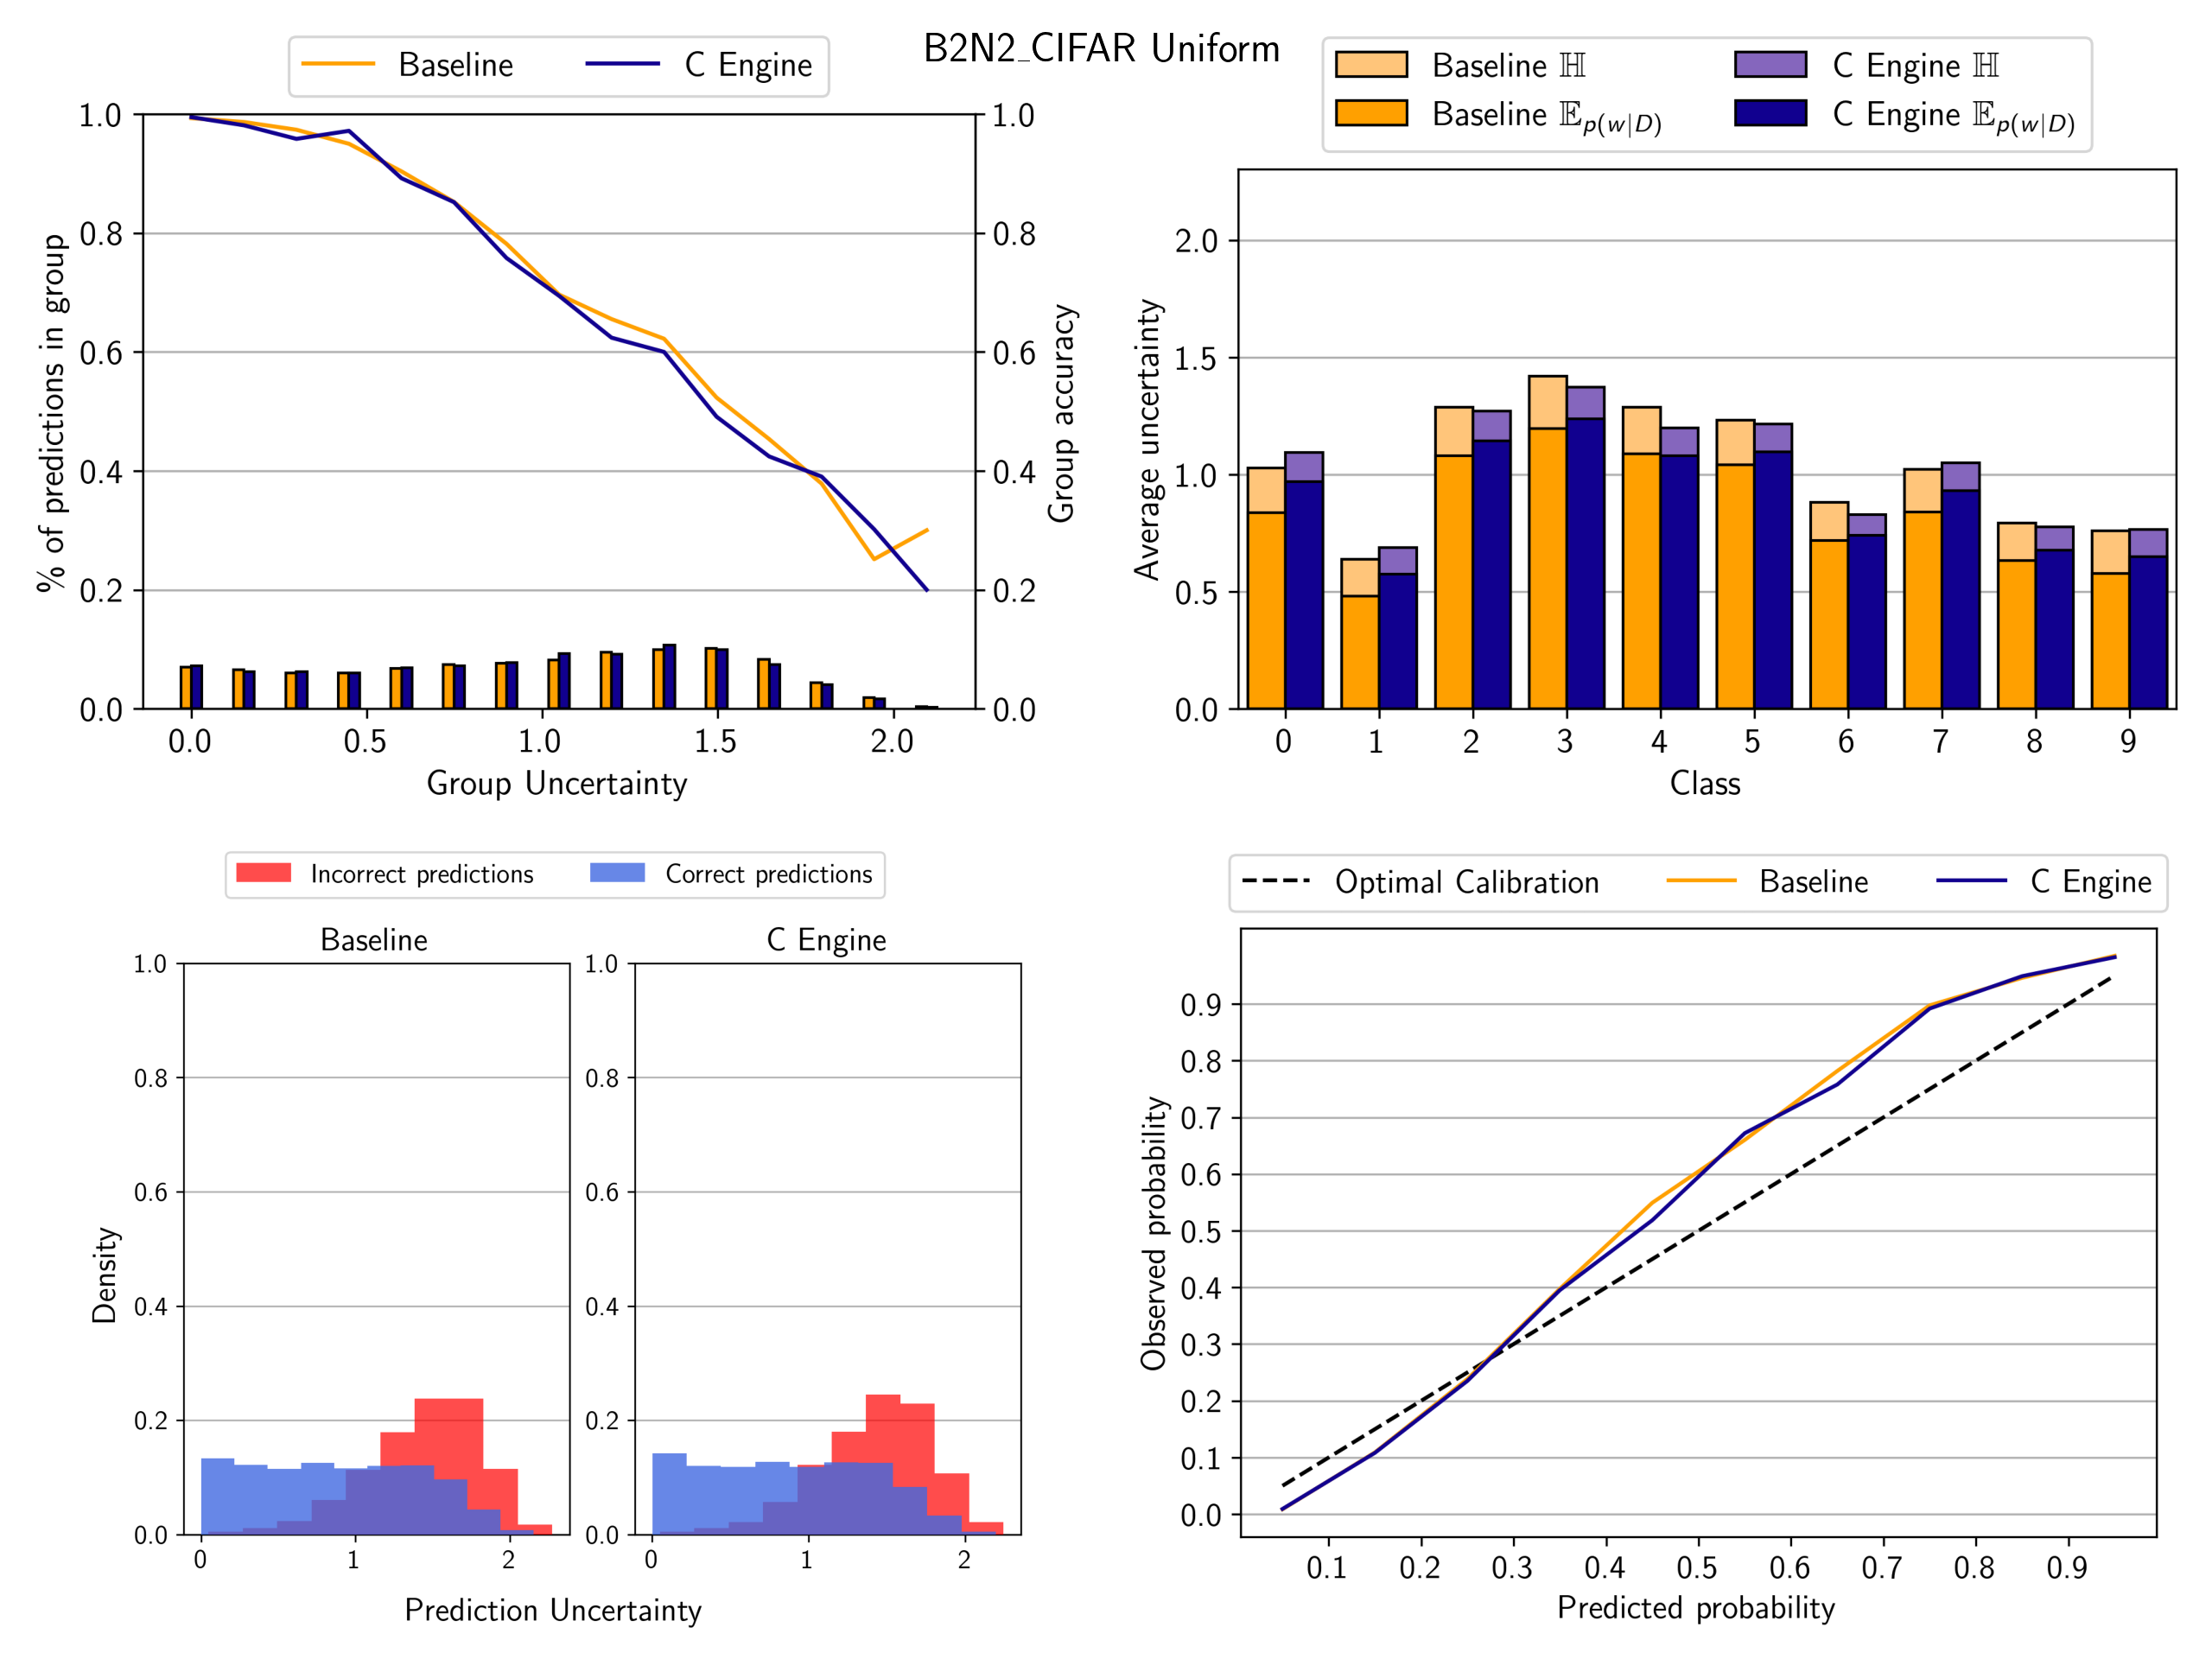
\includegraphics[width=0.9\textwidth]{root/Imagenes/anexo/Uniform-B2N2_CIFAR-mosaic.png}
    \caption{Predicciones del modelo B2N2 con el conjunto de datos CIFAR-10.}
    \label{fig:anx-Uniform-B2N2_CIFAR}
\end{figure}

